\documentclass[../main.tex]{subfiles}

\begin{document}

This project is estimated to last a semester. During this period, a full-time engineer will be hired to carry out all the software development. The estimated cost associated to this position is $30$\euro/hour, taxes included. Considering that during the span of 6 months $37.5 \si{\hour/week}$ of labour will be dedicated to the project, the engineer will work a total of $900 \si{\hour}$.

The development of the project will be carried out on a laptop for convenience. This laptop must have enough computational power to run small tests, but the intensive testing will be carried out in a high-end workstation. An amortisation time of 3 years was considered for these electronic devices. Additionally, the developer will be benefited from a paid subscription to GitHub Pro. All these expenses make up for the material resources listed in Table \ref{tab:b:budget}. These prices were accounted with the \gls{vat} excluded, as this is accounted separately for the entire project.

This work will take place inside \gls{cnb}-\gls{csic} facilities. This research centre not only provides office space for the worker, but it also provides a data centre with adequate cooling and power management for our computing equipment. These costs were accounted as indirect costs, which are $15 \si{\percent}$ of the direct costs. \Gls{cnb}-\gls{csic} is a non-profit organisation. Thus, no industrial benefit will be applied to the budget.

Finally, according to the Spanish economic framework, a $21 \si{\percent}$ \gls{vat} tax was applied to the subtotal. At the end, the budget for this project totals \textbf{THIRTY-NINE THOUSAND THREE HUNDRED THIRTY-EIGHT AND ONE TENTH EUROS} ($39338.10$\euro)

\begin{table}[htbp]
    \centering
    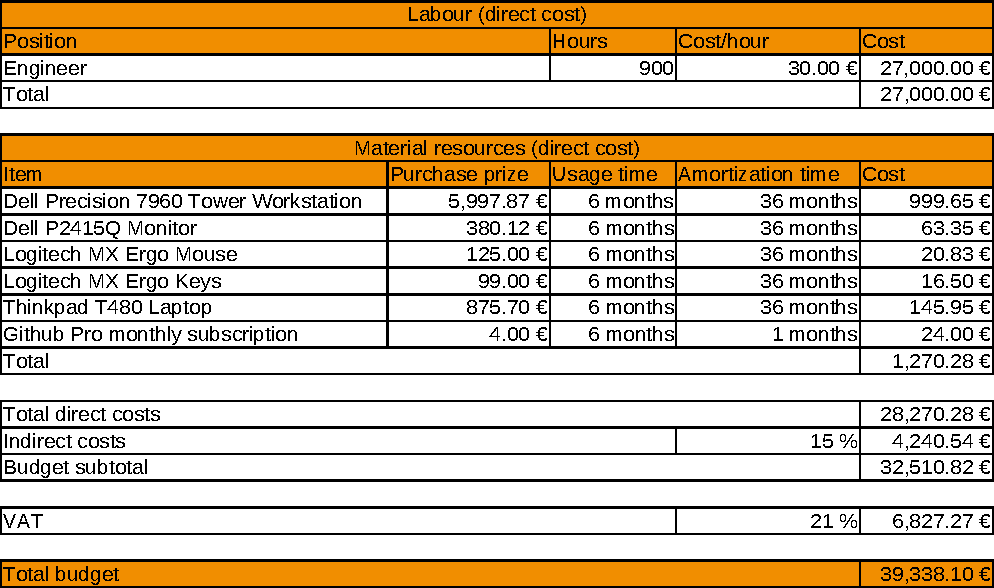
\includegraphics[width=\textwidth]{budget}
    \caption{Budget}
    \label{tab:b:budget}
\end{table}

\end{document}
